\vspace{-2em}
\section{Inductive Analysis}

Recursion employs techniques of repeatedly shrinking the problem to solve its smaller halves. Often found in sorting problems, processing trees, and
geometric problems.

\begin{theo}[MergeSort]
    
    Given an array $A$ of size $n$, we sort via the following:
    \begin{enumerate}
        \item [(i.)] Recursively: Split the array into two halves and wait for a return.
        \item [(ii.)] Base-case: If the array has one element, return it.
        \item [(iii.)] Merge: receive two halves and merge them.
    \end{enumerate}
    The final result is a sorted array.
\end{theo}

\begin{theo}[QuickSort]

    Given an array $A$ of size $n$, we sort via the following:
    \begin{enumerate}
        \item [(i.)] Choose a pivot, set $i$ to the start and $j$ at the end of the array.
        \item [(ii.)] Increase $i$ until $A[i]>pivot$ and decrease $j$ until $A[j]<pivot$.
        \begin{itemize}
            \item If $A[i]<A[j]$, swap $A[i]$ and $A[j]$.
            \item Repeat until $i>j$, return $j$ as the new pivot.
        \end{itemize}
        \item [(iii.)] The new pivot creates two sub-arrays, repeat the process on each sub-array.
    \end{enumerate}
    The final result is $A$ sorted in-place (on the original array without a temporary helper array).
\end{theo}

\begin{Tip} Demos for 
 \textbf{MergeSort}: \url{https://youtu.be/ZLBmc0qf174?si=2b0Kxy9xxPHos_6A} and\\
 \textbf{QuickSort}: \url{https://youtu.be/FWWqLJIUFZM?si=ZPhuvIduWAGXH_mv}.
\end{Tip}

\newpage

\begin{Func}[Mergesort - \texttt{MSORT(A)}]
    \textbf{Input:} Array $A$ and temporary array $temp$ of $n$ elements.\\
    \textbf{Output:} Nothing is returned, the array $A$ is sorted by reference.\\

    \vspace{-.5em}
    \noindent
    \textbf{MSORT function}\textit{(A,temp,i,j)}:\\
    \begin{algorithm}[H]
        \label{algo:mergesort}
        \If{$i \geq j$}{
            \Return;
        }
            $mid \gets (i + j) / 2$\;
            $MSORT(A, temp, i, mid);$ \tcp{Left subarray}
            $MSORT(A, temp, mid + 1, j);$ \tcp{Right subarray}
            $merge(A, temp, i, mid, mid + 1, j);$ \tcp{Merge both halves}
        
    \end{algorithm}

    \vspace{.5em}

    \noindent
    \textbf{Merge function}\textit{(A,temp,i,leftEnd,j,rightEnd)}:\\
    \begin{algorithm}[H]
        $i \gets lefti$; \tcp{Left subarray}
        $j \gets righti$; \tcp{Right subarray}
        $k \gets lefti$; \tcp{Temporary array}
        
        \While{$i \leq leftEnd \ \mathbf{and}\ j \leq rightEnd$}{
            \If{$A[i] < A[j]$}{
                $temp[k] \gets A[i]$; $i \gets i + 1$\;
            } \Else{
                $temp[k] \gets A[j]$; $j \gets j + 1$\;
            }
            $k \gets k + 1$\;
        }
        
        \While{$i \leq leftEnd$}{
            $temp[k] \gets A[i]$; $i \gets i + 1$\; $k \gets k + 1$\;
        }
        
        \While{$j \leq rightEnd$}{
            $temp[k] \gets A[j]$; $j \gets j + 1$\; $k \gets k + 1$\;
        }
        
        \For{$i = lefti$ \textbf{to} $rightEnd$}{
            $A[i] \gets temp[i]$; \tcp{Copy back sorted elements}
        }
    \end{algorithm}

    \noindent\rule{\textwidth}{0.4pt}

    \noindent
    \textbf{Time Complexity:} $O(n \log n)$ in all cases.\\
    \textbf{Space Complexity:} $O(n \log n)$ for the temporary array and $O(\log n)$ for the recursion stack.
\end{Func}

\newpage 

\noindent
Below is a graphical representation of merge sort:
\begin{figure}[h]
    \hspace{-9em}
        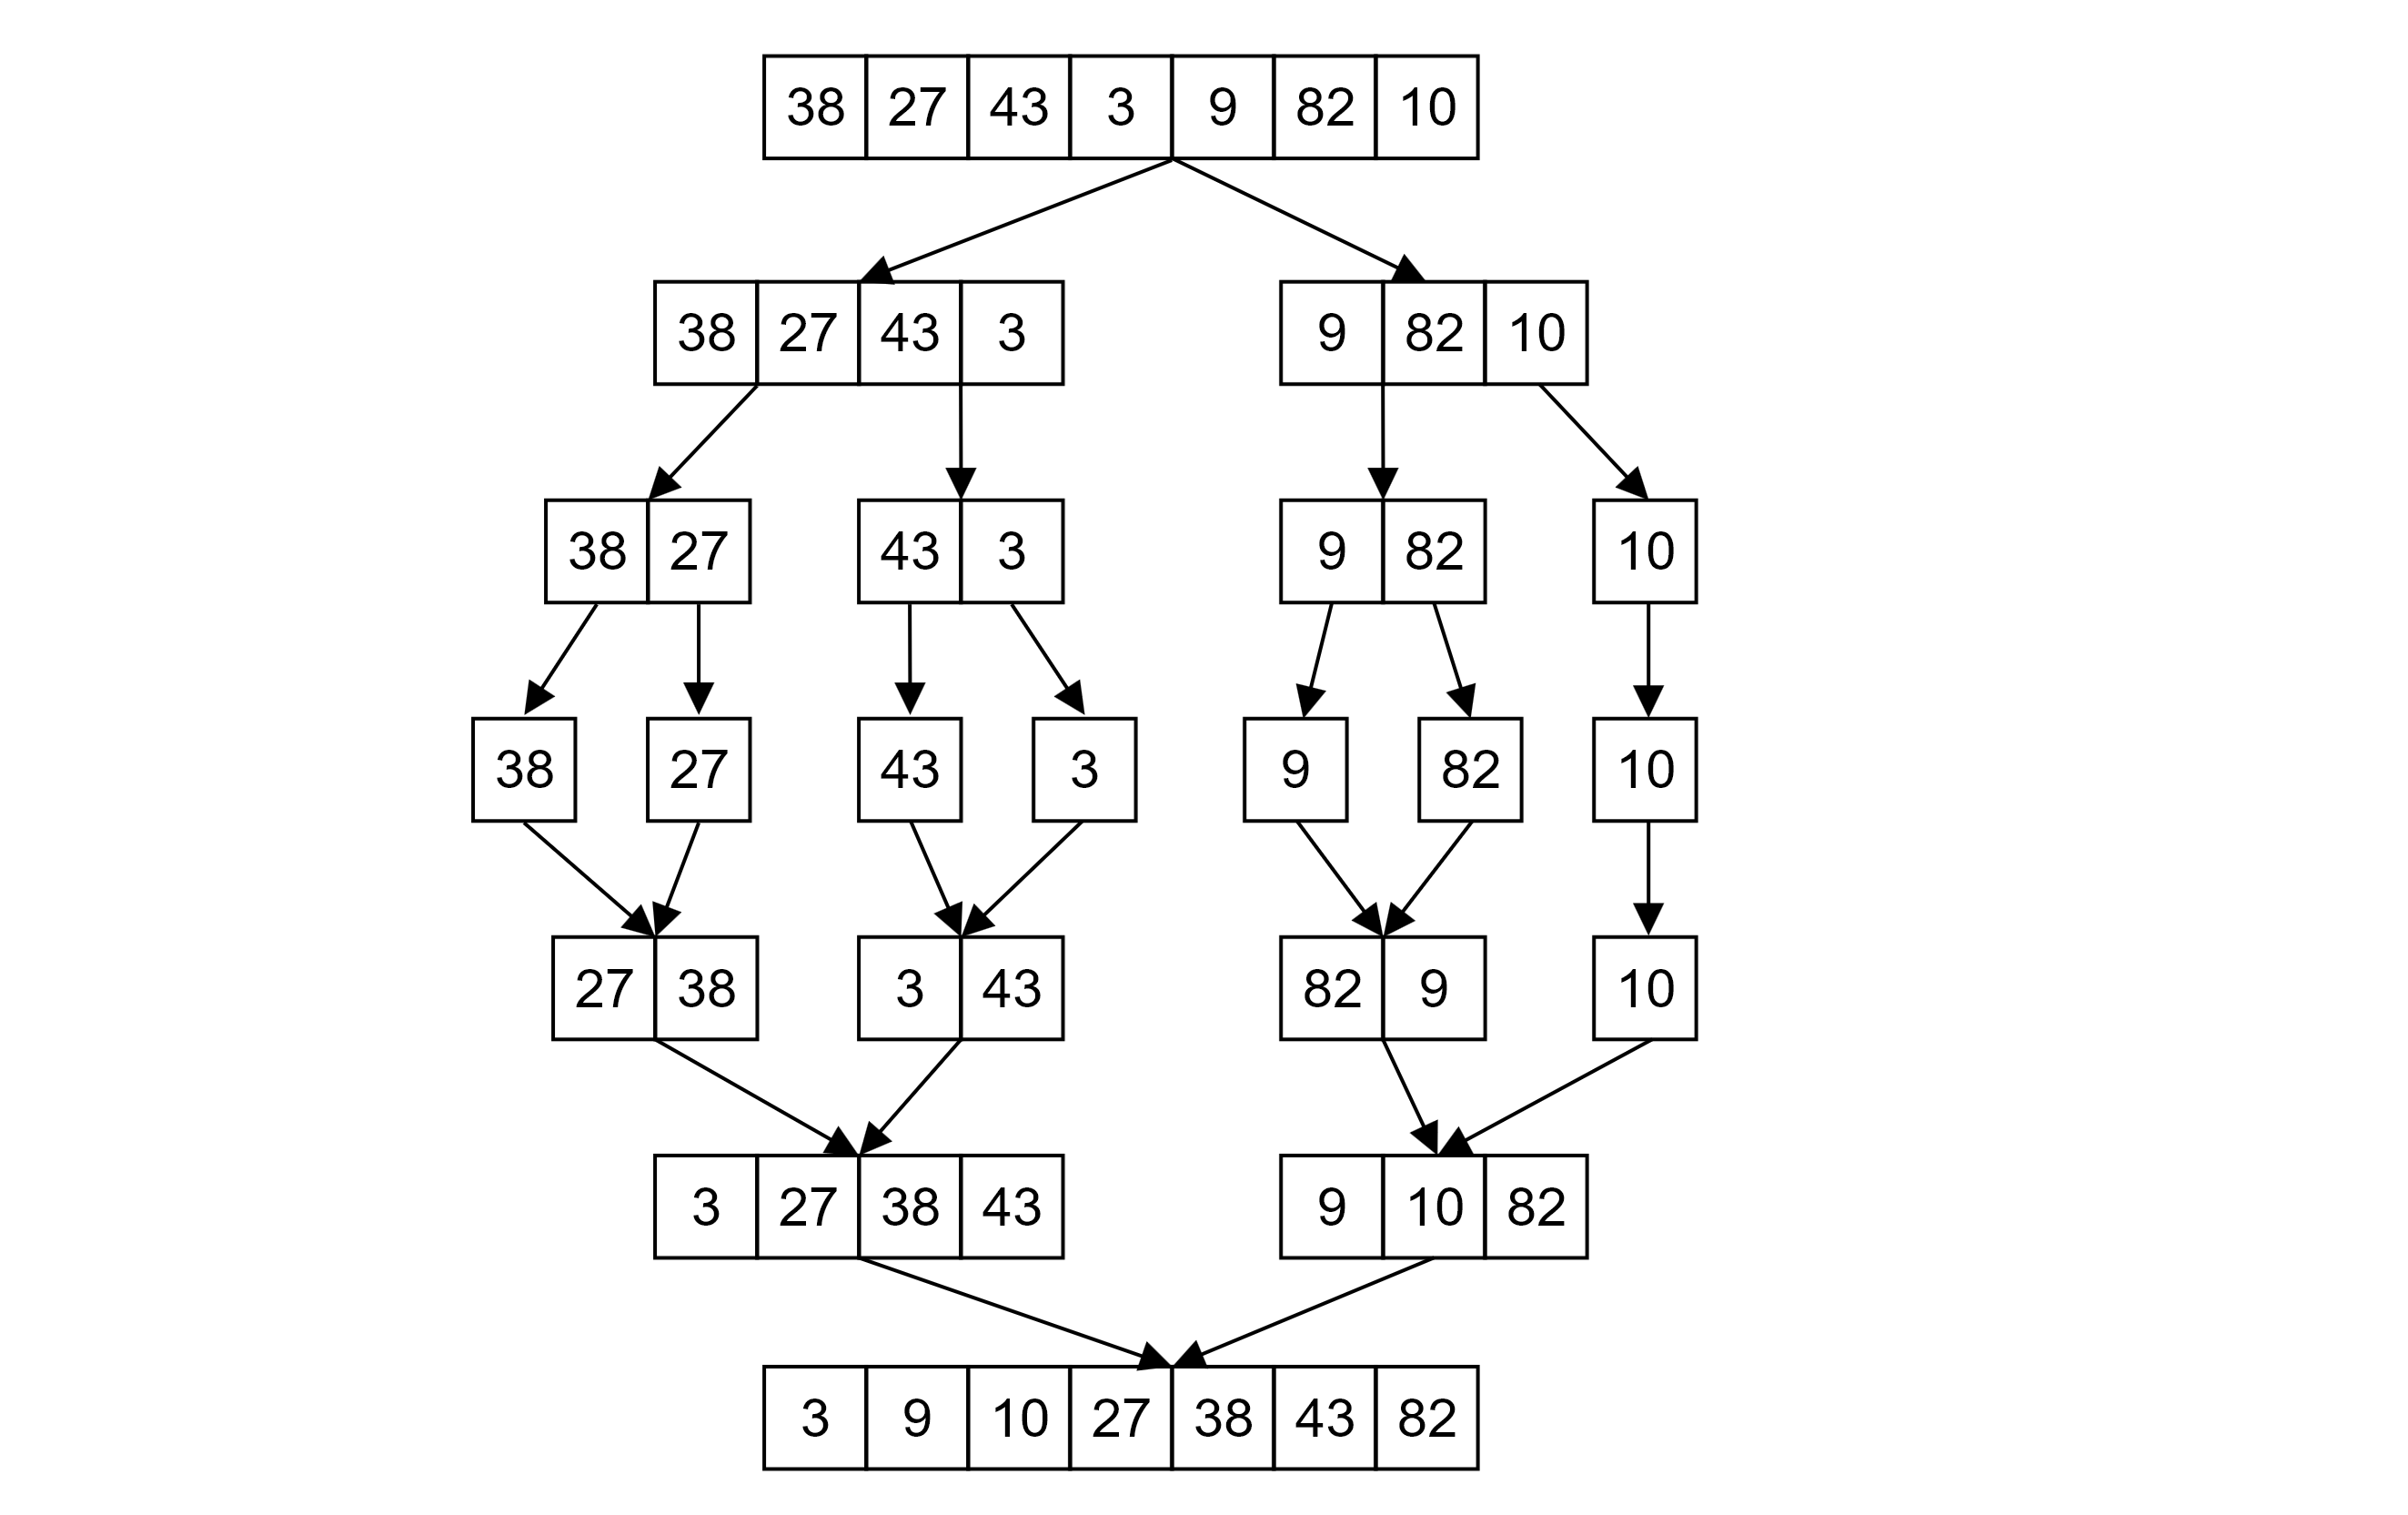
\includegraphics[width=1.5\textwidth]{sections/recurs/mergesort.png}
        \caption{Here is an array of 7 elements. The first partition happens on index 3 as $\left\lfloor (0 + 6)/2 \right\rfloor = 3$. This continues all the way down until we hit our base case;
        During the merge step, we take a temporary array and fill in the missing elements from the two joining halves. Here the next smallest element is picked from 
        each half, if one finishes first, we copy the rest of the other half into the temporary array. Finally, we copy back the temporary array to the original array.}
\end{figure}


\newpage 

\begin{Func}[Quicksort - \texttt{QSORT(A,high,low)}]
    \textbf{Input:} Array $A$ of $n$ elements.\\
    \textbf{Output:} Sorted array $A$ in ascending order.\\
    \textbf{Initial Call:} $QSORT(A, 0, n-1)$\\

    \vspace{-.5em}
    \noindent
    \textbf{QSORT function}\textit{(A,low,high)}\\
    \begin{algorithm}[H]
        \label{algo:quicksort}
        \If{$low < high$}{
            $pivot \gets \texttt{partition}(A, low, high)$\;
            $QSORT(A, low, pivot);$ \tcp{Left of the pivot}
            $QSORT(A, pivot + 1, high);$ \tcp{Right of the pivot}
        }
    \end{algorithm}

    \vspace{.5em}

    \noindent
    \textbf{Partition function}\textit{(A,low,high)}:\\
    \begin{algorithm}[H]
        $pivot \gets A[\left\lfloor (low + high)/2 \right\rfloor]$\;
        $i \gets low - 1$\;
        $j \gets high + 1$\;
        
        \While{$i < j$}{
            \Repeat{$i \gets i + 1$}{
                \If{$A[i] \geq pivot$}{
                    \textbf{break};
                }
            }
            \Repeat{$j \gets j - 1$}{
                \If{$A[j] \leq pivot$}{
                    \textbf{break};
                }
            }
            \If{$i < j$}{
                $A.swap(i, j)$;
            }
        }
        \KwRet{$j$}; \tcp{Return the index of the partition}
    \end{algorithm}

    \noindent\rule{\textwidth}{0.4pt}

    \noindent
    \textbf{Time Complexity:} Average case $O(n \log n)$, Worst case $O(n^2)$.\\
    \textbf{Space Complexity:} $O(n)$ for input. The sorting is done in place, and the recursion stack takes $O(\log n)$ space in the average case. Worst case space complexity is $O(n)$.
\end{Func}


\vspace{-1em}
\begin{theo}[Worst Cases - Merge and Quick Sort]

    \begin{itemize}
        \item \textbf{Merge Sort:} independent of the input, always $O(n \log n)$.
        \vspace{-.5em}
        \item \textbf{Quick Sort:} If the array is sorted in ascending/descending order, the pivot is the smallest/largest element, respectively. This results in $O(n^2)$ time complexity, as each partition is of size $n-1$.
    \end{itemize}
\end{theo}

\newpage 

\noindent
Let us examine merge sort at a high-level.
\begin{Func}[Mergesort - \texttt{MSORT(A)}]
    \textbf{Input:} Array $A$ and temporary array $temp$ of $n$ elements.\\
    \textbf{Output:} Nothing is returned, the array $A$ is sorted by reference.\\

    \vspace{-.5em}
    \noindent
    \textbf{MSORT function:}\\
    \begin{algorithm}[H]
        \label{algo:mergesort}
        \If{$i \geq j$}{
            \Return;
        }
            $mid \gets (i + j) / 2$\;
            $MSORT(A, temp, i, mid);$ \tcp{Left subarray}
            $MSORT(A, temp, mid + 1, j);$ \tcp{Right subarray}
            $merge(A, temp, i, mid, mid + 1, j);$ \tcp{Merge both halves}
        
    \end{algorithm}
\end{Func}

\begin{Proof}[Merge Sort - Time Complexity]

    \label{proof:merge}
We make the following observations, generalizing $n$ to each recursive call:
\begin{enumerate}
    \item [(i.)] We make 2 recursive calls.
    \item [(ii.)] Each recursive call cuts the array in half, $n/2$.
    \item [(iii.)] We do $\Theta(n)$ work to merge the two halves, returning up the stack.
\end{enumerate}
\noindent
We define a general form for our traversals as function $T(n)$:\\


    \hspace{-4em}
    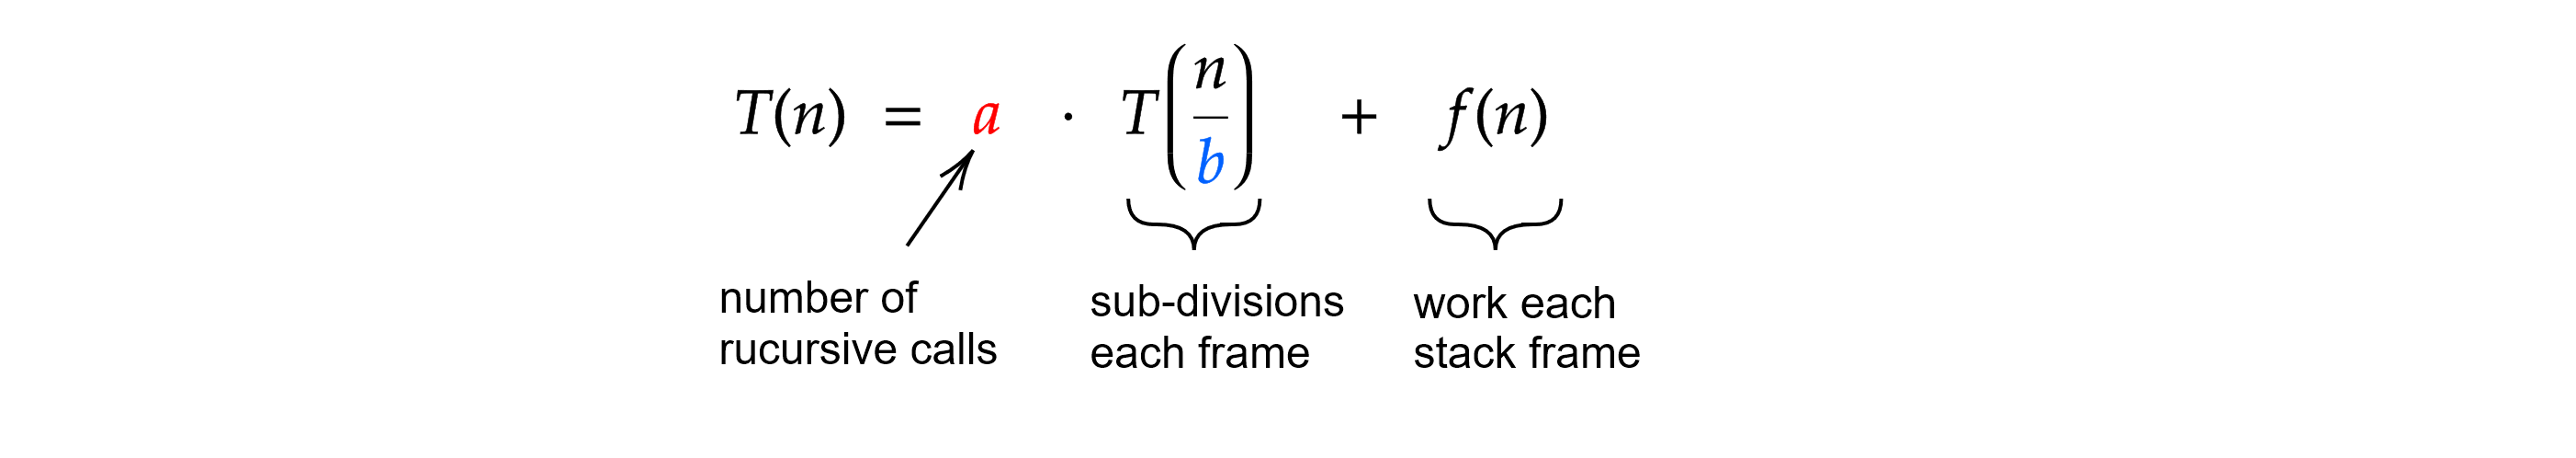
\includegraphics[width=1.2\textwidth]{sections/recurs/rec_form.png}

   
\noindent
For merge sort, we have $T(n) = 2\cdot T(n/2) + \Theta(n)$. This means we i with input $T(n)$ and then 
our first recursive call is $T(n/2)$, the calls from there are $T(n/4)$, $T(n/8)$, and so on. Therefore,
at any given layer $k$, we have $2^k$ calls, with each input $T(n/2^k)$. We stop when $n/2^k = 1$, which is $k = \log n$. Since $2^{\log_2 n} = n$, then $\left(\dfrac{n}{2^{\log_2 n}}\right) = 1$.
Thus, the depth of our recursion is $\log n$, and $n$ work is done when unraveling the stack, hence $O(n \log n)$.

\end{Proof}

\newpage

\noindent
To illustrate the above proof, we can draw a recursion tree for merge sort:\\
\vspace{-5em}
\begin{figure}[h]
    \hspace{-12em}
    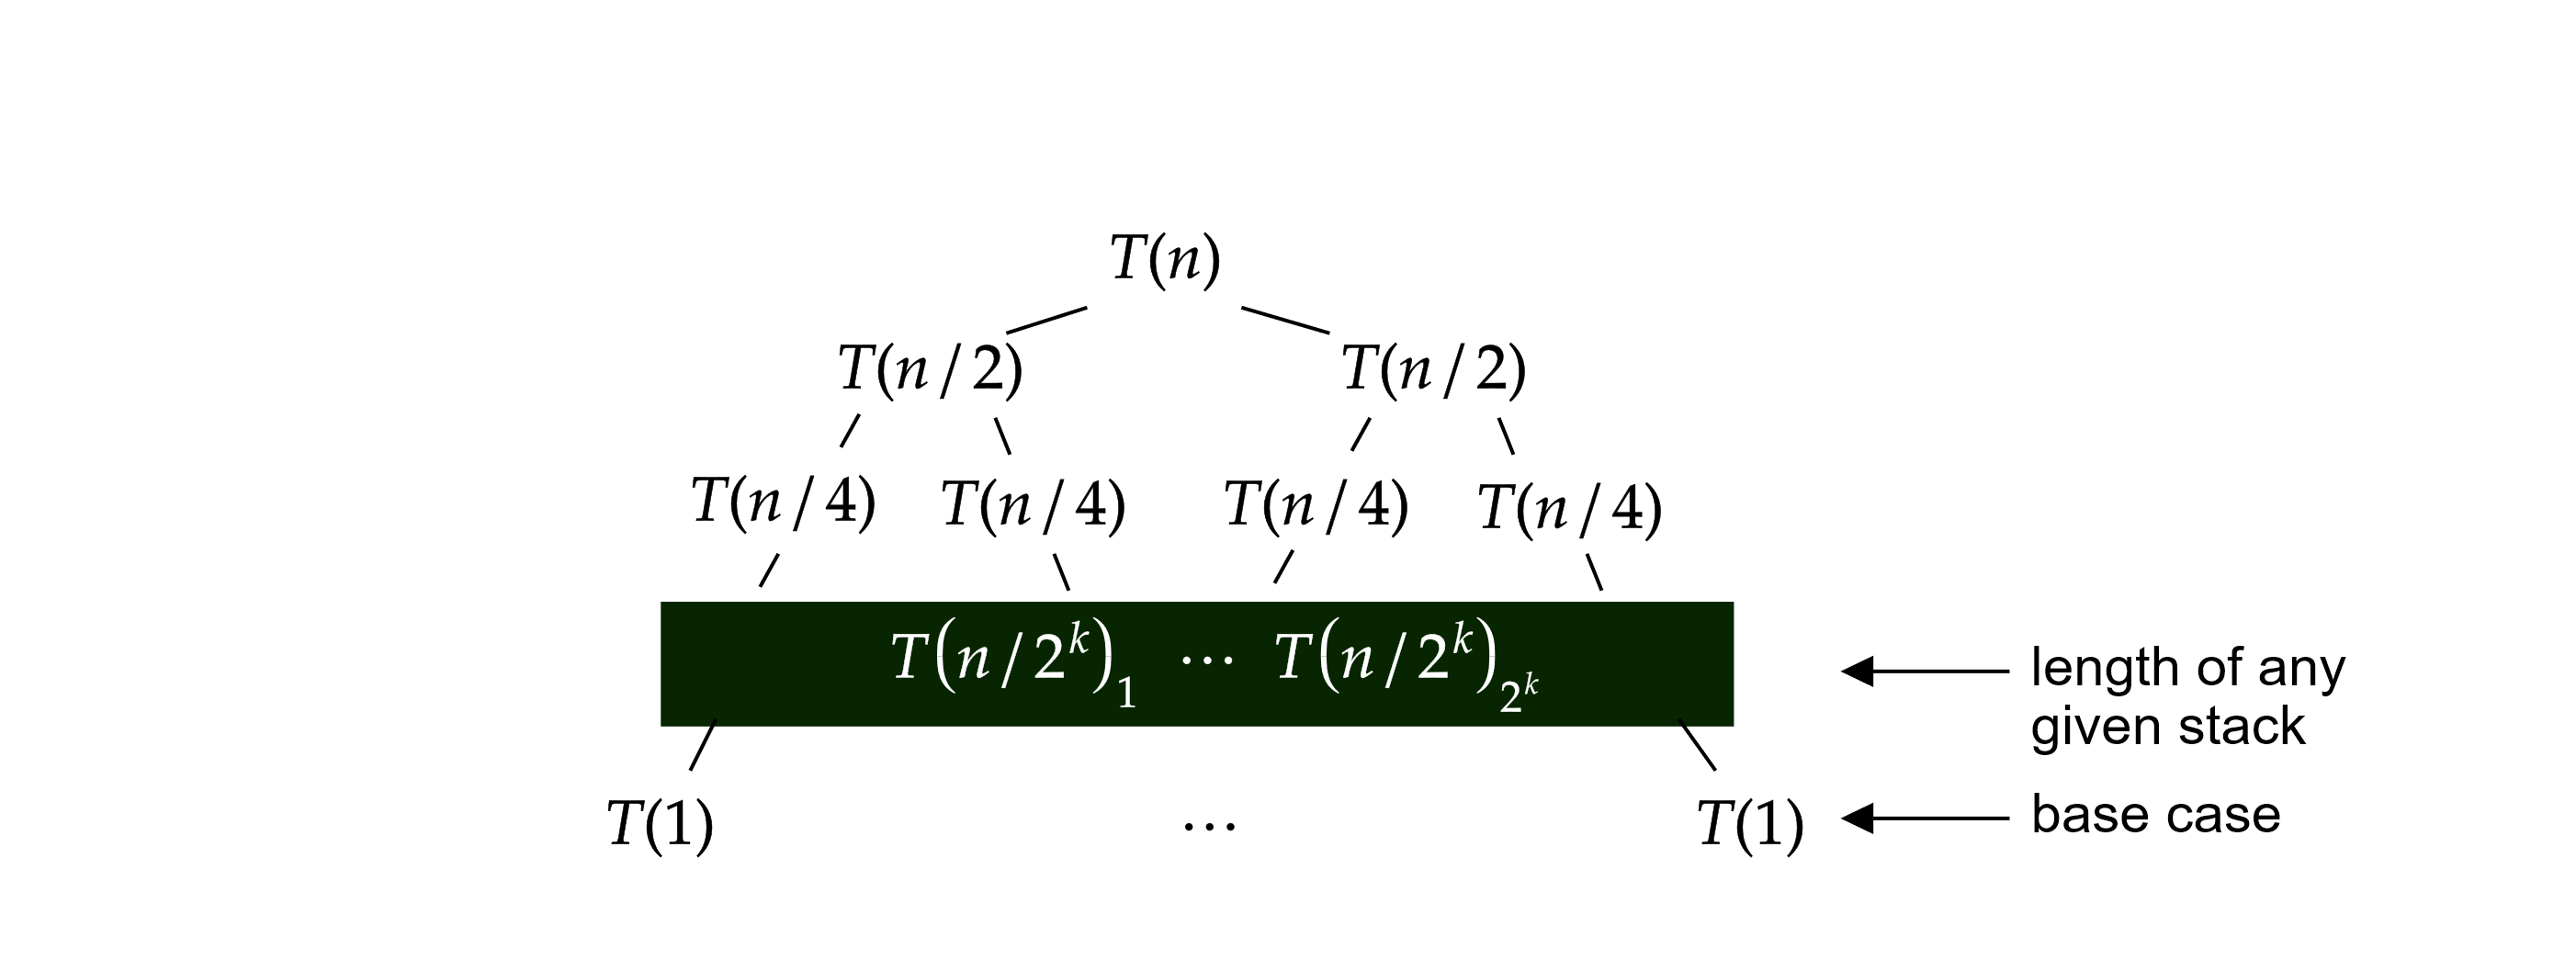
\includegraphics[width=1.5\textwidth]{sections/recurs/rec_tree.png}
    \caption{Recursion Tree for Merge Sort}
\end{figure}

\vspace{-1em}
\begin{Func}[Quicksort - \texttt{QSORT(A)}]
    \textbf{Input:} Array $A$ of $n$ elements.\\
    \textbf{Output:} Sorted array $A$ in ascending order.\\

    \vspace{-.5em}
    \noindent
    \textbf{QSORT function:}\\
    \begin{algorithm}[H]
        \label{algo:quicksort}
        \If{$low < high$}{
            $pivotIndex \gets \texttt{partition}(A, low, high)$\;
            $QSORT(A, low, pivotIndex);$ \tcp{Left of the pivot}
            $QSORT(A, pivotIndex+1, high);$ \tcp{Right of the pivot}
        }
    \end{algorithm}
\end{Func}

\vspace{-1em}
\noindent
\begin{Proof}[Quick Sort - Time Complexity]

    First does $\Theta(n)$ work to partition, then makes 2 recursive calls, and each recursive call 
    has on average $n/2$ elements. We define a general form for our traversals as function $2T(n/2) + \Theta(n)$.
    Thus $\log n$ levels of recursion, each taking $\Theta(n)$ time to partition, hence $O(n \log n)$.\\

    \noindent
    In worst case, $2T(n-1) + \Theta(n)$. Then we have $n$ levels of recursion, each taking $\Theta(n)$ time to partition, hence $O(n^2)$.

\end{Proof}

\newpage

\begin{theo}[Proving Correctness of Recursive Functions]

    To prove correctness of a recursive function, we need to show:
    \begin{enumerate}
        \item \textbf{Base Case:} The base case is correct.
        \item \textbf{Inductive Hypothesis:} Assume $k$ input sizes are correct, where $k<n$, we assume 
        the recursive calls return the correct result.
        \item \textbf{Inductive Step:} Show that the problem reduces to the base case, and that intermediate steps other than the recursive calls are correct.
    \end{enumerate}
    If all three conditions are met, then the function is correct for all $n$.
\end{theo}

\begin{theo}[Master Method for Recursive Time Complexity]

    \label{theo:master}

    The master method is a general technique for solving recurrences of the form:
    \begin{equation*}
        T(n) = \textcolor{red}{a}T\left(\dfrac{n}{\textcolor{blue}{b}}\right) + f(n^{\textcolor{OliveGreen}{d}})
        \end{equation*}
        where $\textcolor{red}{a} \geq 1$, $\textcolor{blue}{b} > 1$, and $f(n)$ is a given function. We consider degree $\textcolor{OliveGreen}{d}$ of $f(n)$:
        \begin{align*}
        \textcolor{OliveGreen}{d} > \log_{\textcolor{blue}{b}} \textcolor{red}{a} &\implies T(n) = \Theta(n^{\textcolor{OliveGreen}{d}}) \\
        \textcolor{OliveGreen}{d} < \log_{\textcolor{blue}{b}} \textcolor{red}{a} &\implies T(n) = \Theta(n^{\log_{\textcolor{blue}{b}} \textcolor{red}{a}}) \\
        \textcolor{OliveGreen}{d} = \log_{\textcolor{blue}{b}} \textcolor{red}{a} &\implies T(n) = \Theta(n^{\log_{\textcolor{blue}{b}} \textcolor{red}{a}} \log n)
        \end{align*}
    
\end{theo}

\begin{Tip}
    Extended Version of the Master Method:
    \\ $$T(n) = f(n) + \sum_{i=1}^{k} a_i T(b_i n + h_i(n))$$
    where  $h_i(n) = O\left( \frac{n}{\log^2 n} \right)$. This is the \textbf{Akra-Bazzi Method}:\\
    Link: \url{https://en.wikipedia.org/wiki/Akra%E2%80%93Bazzi_method}.
\end{Tip}

\textbf{Examples:}
\begin{itemize}
    \item $T(n) = 2T\left(\frac{n}{2}\right) + n^3$: ($a=2$; $b=2$; $d=3$;) then ($\log_2 2 = 1 < 3$) hence $T(n) = \Theta(n^3)$.
    \item $T(n) = 5T\left(\frac{n}{2}\right) + n^2$: ($a=5$; $b=2$; $d=2$;) then ($\log_2 5 \approx 2.32 > 2$) hence $T(n) = \Theta(n^{\log_2 5})$
    \item $T(n) = 16T\left(\frac{n}{4}\right) + n^2$: We have $d:=2$ and ($log_4 16=2=d$) hence $T(n) = \Theta(n^{log_4 16}\log n)$ 
\end{itemize}

\newpage

\begin{Func}[Mergesort - \texttt{MSORT(A)}]
    \textbf{Input:} Array $A$ and temporary array $temp$ of $n$ elements.\\
    \textbf{Output:} Nothing is returned, the array $A$ is sorted by reference.\\

    \vspace{-.5em}
    \noindent
    \textbf{MSORT function:}\\
    \begin{algorithm}[H]
        \label{algo:mergesort}
        \If{$i \geq j$}{
            \Return;
        }
            $mid \gets (i + j) / 2$\;
            $MSORT(A, temp, i, mid);$ \tcp{Left subarray}
            $MSORT(A, temp, mid + 1, j);$ \tcp{Right subarray}
            $merge(A, temp, i, mid, mid + 1, j);$ \tcp{Merge both halves}
        
    \end{algorithm}
\end{Func}

\vspace{-1.5em}
\begin{Proof}[Correctness of Merge Sort]

    By strong induction on the input size $n$:
    
    \begin{enumerate}
        \item \textbf{Base Case:}  
        If $i \geq j$, then the array is of size 1, and is already sorted.
        
        \item \textbf{Inductive Hypothesis:}  
        Assume that Merge Sort correctly sorts arrays of sizes $k$ where $1\leq k < n$.
        
        \item \textbf{Inductive Step:}  
        Our two recursive calls follow, 
        \begin{enumerate}
        \item[(i.)] $mid \gets \floor{(i + j) / 2}$
        \item[(ii.)] $MSORT(A, temp, i, mid)$
        \item[(iii.)] $MSORT(A, temp, mid + 1, j)$
        \end{enumerate}
    \end{enumerate}
    \noindent
    Suppose (ii.) and (iii.) do not reach the base case. Then in (ii.) $mid>=j$ and in (iii.) $mid+1<=i$, which contradicts, as
    $mid:=\floor{(i+j)/2}$, then $i\leq mid \leq j$.\\

    \vspace{-4em}
    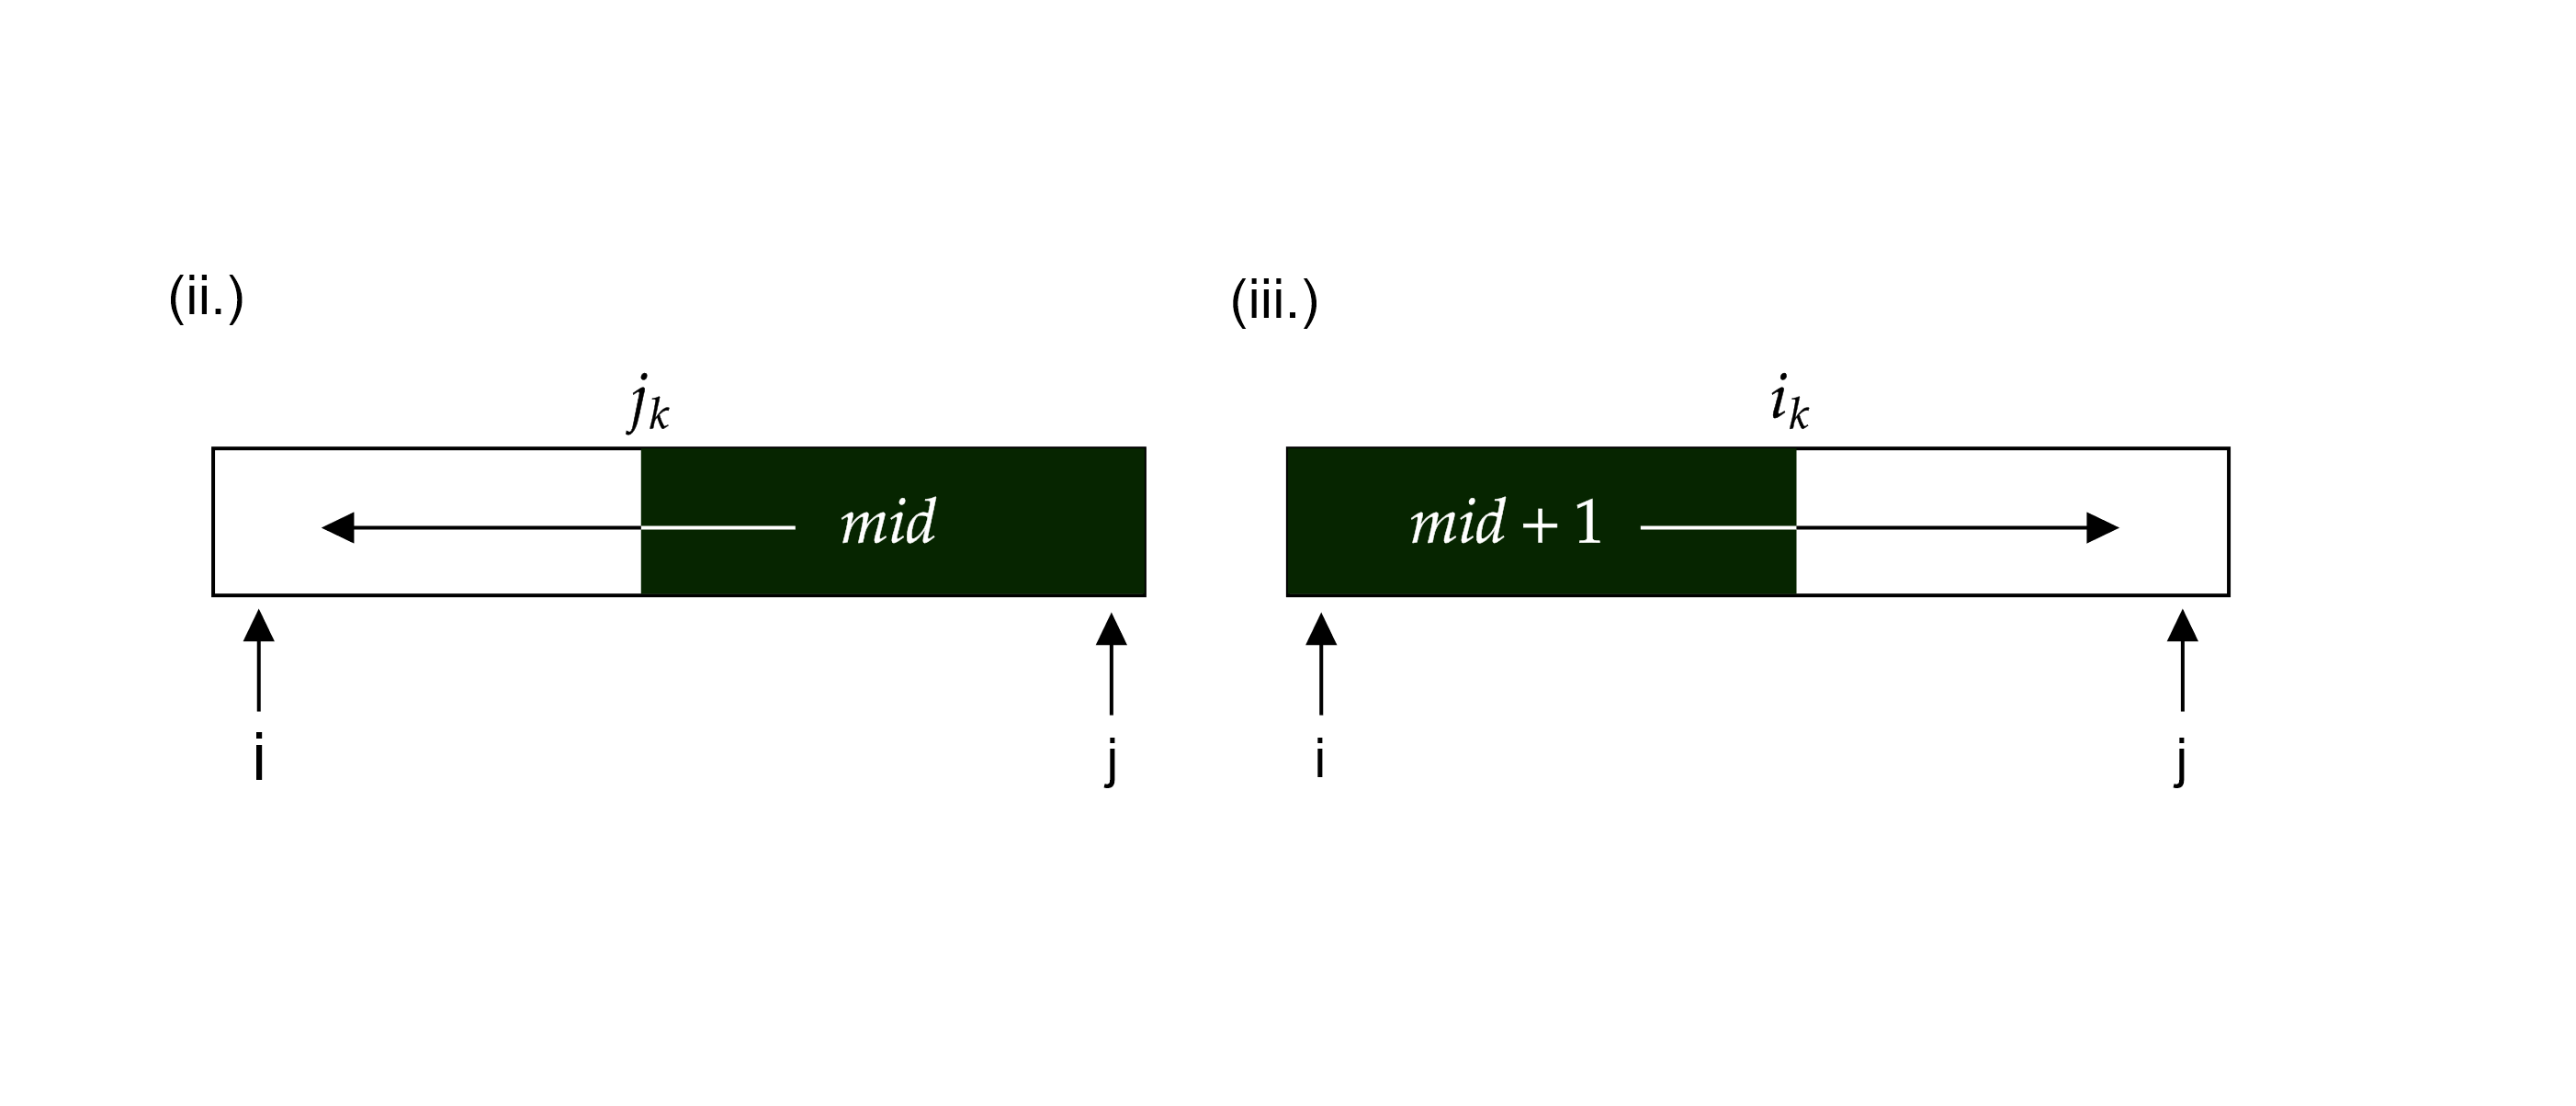
\includegraphics[width=1\textwidth]{sections/recurs/msort_proof.png}

    \vspace{-4em}
    \noindent
    Then in (ii.), the right bound $mid$ keeps decreasing, and in (iii.), the left bound $mid$ keeps increasing.
    This shirks both sub-arrays until both bounds meet. The merge function sorts after both calls, taking the next 
    biggest in the sub-arrays, placing it in the temporary array, and copying back to the original array. Hence, by induction, the function is correct.
\end{Proof}

\newpage

\begin{theo}[Iterative Substitution Method (plug-and-chug)]

    \label{theo:iterative}

    Given a function $T(n)$ which has a recurrence relation---meaning it calls 
    upon itself in its own definition---we may repeatedly substitute such self-references
    back into $T(n)$.

    Given that $T(n)$ properly subdivides to a base case $T(x)$, we may derive some
    pattern which illustrates the state of $T(n)$ at some depth $k$ within the recurrence.
    Doing so, we identify what makes our $k_{th}$ expression hit $T(x)$.
\end{theo}
\begin{Proof}[Iterative Substitution Method (plug-and-chug) - MergeSort]

    \vspace{-.5em}
    Merge sort has the recurrence relation $T(n) = 2T(n/2) + \Theta(n)$, for which the base case is $T(1)$.
    We substitute $T(n/2)$ into $T(n)$:
    \begin{align*}
        T(n) &= 2T(n/2) + \Theta(n);\quad \text{ and }\quad T(n/2) = 2T(n/2^2) + \Theta(n/2);\\
        T(n) &= 2\left[\hspace{3em} \right] + \Theta(n)\text{; Prepare to substitute the recurrence $T(n/2)$}\\
         &= 2\left[2T(n/2^2) + \Theta(n/2)\right] + \Theta(n);\text{ we evaluate $2\cdot\Theta\left(n/2\right)$ as $\Theta\left(2n/2\right)$}\\
         &= 2^2T(n/2^2) + \Theta(n) + \Theta(n)\text{; Simplified}\\
    \end{align*}

    \vspace{-1.5em}
\noindent
We won't fully simplify to observe how the recurrence builds. We continue, evaluating $T(n/2^2)$:
\begin{align*}
    T(n/2^2) &= 2T(n/2^3) + \Theta(n);\\
    T(n) &= 2^2\left[2T(n/2^3) + \Theta(n/2^2)\right] + \Theta(n)+\Theta(n);\text{substitute again}\\
    &= 2^3T(n/2^3) + \Theta(n)+\Theta(n)+\Theta(n)\text{; Simplified}\\
\end{align*}

\vspace{-1.5em}
\noindent
We identify the pattern for the $k_{th}$ substitution:
\begin{align*}
    T(n) &= 2^kT(n/2^k) + k\cdot\Theta(n)\text{; General form}\\
\end{align*}

\vspace{-1.5em}
\noindent
Now we identify what makes our recurrence $T(n/2^k) = T(1)$, i.e., where is $n/2^k = 1$, then $n=2^k$, and $\log_2 n = k$. We plug this back into our general form:
\begin{align*}
    T(n) &= 2^{\log_2 n}T(n/2^{\log_2 n}) + \log_2 n\cdot \Theta(n)\text{; Substituting $k$}\\
    &= n\Theta(1) + \log_2 n\cdot\Theta(n);\text{ Where $T(1)=\Theta(1)$}\\
    &= \Theta(n) + \Theta(n)\log_2 n;\\
    &= \Theta(n\log n);
\end{align*}
Hence, merge sort has a time complexity of $O(n\log n)$.
\end{Proof}
\begin{Tip}
    Live Demo: \href{https://youtu.be/AJmDcuU42JY?t=2526}{Evaluating Recursion -- Master Method}
\end{Tip}

\newpage 

\noindent

\subsection{Efficiency of Multiplication: Karatsuba's Algorithm}
Recall Section (\ref{sec:effic}), which discusses manipulating base 2. There is a problem when trying to 
multiply two $n$-bit integers, as we have to compute $n^2$ products, which is inefficient. We can attempt to reduce the number of products by using a divide-and-conquer approach.\\
\[A_1 2^{\ceil{n/2}}+A_0=:a \quad \times \quad b:= B_1 2^{\ceil{n/2}}+B_0.\]
\noindent
Then we have,
\begin{align*}
    a\cdot b &=(A_1 2^{\ceil{n/2}}+A_0)(B_1 2^{\ceil{n/2}}+B_0)\\
    &=(A_1 2^{\ceil{n/2}})(B_1 2^{\ceil{n/2}})+(A_1 2^{\ceil{n/2}})B_0+(B_1 2^{\ceil{n/2}})A_0+A_0B_0\\
    &=(A_1B_1)2^{n}+(A_1B_0+B_1A_0)2^{\ceil{n/2}}+A_0B_0.
\end{align*}
\noindent
We need to compute 4 products, $(A_1B_1)$, $(A_1B_0), (B_1A_0)$, and $(A_0B_0)$. We now attempt to solve them independently:

\begin{Func}[Multiplication of $n$-bit Integers - \textit{Multiply()}]
    Let $a$ and $b$ be $n$-bit integers of base 2. This algorithm recursively computes the product of $a$ and $b$ using a straightforward divide-and-conquer approach.

    \vspace{.5em}
    \noindent
    \textbf{Input:} $n, a, b$ (where $a$ and $b$ are $n$-bit integers)\\
    \textbf{Output:} The product $a \times b$\\

    \begin{algorithm}[H]
        \SetAlgoLined
        \SetKwProg{Fn}{Function}{:}{\KwRet{}}
        \Fn{\textit{Multiply}($n, a, b$)}{
            \If{$n < 2$}{
                \textbf{return} the result of grade-school multiplication for $a \times b$\;
            }
            \Else{
                $A_1 \gets a \div 2^{n/2};\ A_0 \gets a \bmod 2^{n/2}$\;
                $B_1 \gets b \div 2^{n/2};\ B_0 \gets b \bmod 2^{n/2}$\;

                \vspace{.5em}
                $p_1 \gets \textit{Multiply}(n/2, A_1, B_1)$\;
                $p_2 \gets \textit{Multiply}(n/2, A_1, B_0)$\;
                $p_3 \gets \textit{Multiply}(n/2, A_0, B_1)$\;
                $p_4 \gets \textit{Multiply}(n/2, A_0, B_0)$\;

                \textbf{return} $p_1 \cdot 2^n + (p_2 + p_3) \cdot 2^{n/2} + p_4$\;
            }
        }
    \end{algorithm}
    \noindent\rule{\textwidth}{0.4pt}

    \noindent
    \textbf{Time Complexity:} $O(n^2)$, as in our master method $T(n)=4T(n/2)+O(n)$, Theorem (\ref{theo:master}).\\
    \textbf{Space Complexity:} $O(n)$, storing $n+n$ bits for $a$ and $b$, while we track $O(\log_2 n)$ depth in the recursion stack.
\end{Func}


\noindent
As one might of noticed, we didn't improve the time complexity whatsoever. This is where we employ a clever mathematical trick.
\newpage

\label{page:karatsuba}
\noindent
Observe the full term, $c:=(\textcolor{red}{A_1B_1})2^{n}+(\textcolor{blue}{A_1B_0+B_1A_0})2^{\ceil{n/2}}+\textcolor{red}{A_0B_0}.$ Say we computed some term,
\[z:=(A_1+A_0)(B_1+B_0)=(\textcolor{red}{A_1B_1})+\textcolor{blue}{(A_1B_0)+(B_1A_0)}+(\textcolor{red}{A_0B_0}).\]
\noindent
Notice how $z$ also contains $(A_1B_1)$ and $(A_0B_0)$, which are also in $c$. Say
$m=(A_1B_0)+(B_1A_0)$. Let $x:=(A_1B_1)$ and $y:=(A_0B_0)$ then $z-x-y=m$. This reduces the number of multiplications to 3, as we only compute
 $(A_1B_1)$, $(A_0B_0)$ once, and then $z$.\\

\noindent
We employ the above strategy, which is \textbf{Karatsuba's multiplication algorithm}:

\begin{Func}[Karatsuba's Multiplication Algorithm - \textit{KMul()}]
    Let $a$ and $b$ be $n$-bit integers of base 2. This algorithm recursively computes the product of $a$ and $b$ using a divide-and-conquer approach.

    \vspace{.5em}
    \noindent
    \textbf{Input:} $n, a, b$ (where $a$ and $b$ are $n$-bit integers)\\
    \textbf{Output:} The product $a \times b$\\

    \begin{algorithm}[H]
        \SetAlgoLined
        \SetKwProg{Fn}{Function}{:}{\KwRet{}}
        \Fn{\textit{Multiply}($n, a, b$)}{
            \If{$n < 2$}{
                \textbf{return} the result of grade-school multiplication for $a \times b$\;
            }
            \Else{
                $A_1 \gets a \div 2^{n/2};\ A_0 \gets a \bmod 2^{n/2}$\;
                $B_1 \gets b \div 2^{n/2};\ B_0 \gets b \bmod 2^{n/2}$\;

                \vspace{.5em}
                $x \gets \textit{Multiply}(n/2, A_1, B_1)$\;
                $y \gets \textit{Multiply}(n/2, A_0, B_0)$\;
                $z \gets \textit{Multiply}(n/2, A_1 + A_0, B_1 + B_0)$\;

                \textbf{return} $x \cdot 2^n + (z - x - y) \cdot 2^{n/2} + y$\;
            }
        }
    \end{algorithm}
    \noindent\rule{\textwidth}{0.4pt}

    \noindent
    \textbf{Time Complexity:} $O(n^{\log_2 3}) \approx O(n^{1.585})$, as in our master method $T(n)=3T(n/2)+O(n)$, Theorem (\ref{theo:master}).\\
    \textbf{Space Complexity:} $O(n)$.
\end{Func}

\newpage 

\begin{Exercise} Evaluate the following functions with the Master Method and Substitution:
    \begin{enumerate}
        \item makes 2 recursive calls, recursive calls of length $n/3$, and does $\Theta(n)$ work.
        \item makes 4 recursive calls, recursive calls of length $n/3$, and does $\Theta(n)$ work.
        \item makes 9 recursive calls, recursive calls of length $n/3$, and does $\Theta(n^2)$ work.
    \end{enumerate}
\end{Exercise}

\vspace{-.5em}
\begin{Note}
    \textbf{Note:} Helpful log identities: $\log_a 2b = 2\log_a b$; $a^{\log_a b} = b$; $a^{\log_b c} = c^{\log_b a}$.
\end{Note}

\begin{Exercise} Find the recurrence relation for the below function then solve it:
\end{Exercise}

\vspace{-.5em}
\begin{Func}[Mystery Function - \texttt{MYST(n)}]

    \vspace{-1em}
    \begin{algorithm}[H]
    \If{$n \leq 1$}{
        \Return 1
    }
    \ElseIf{$x > 6$}{
        \Return \texttt{MYST($n/2$)} + $O(n)$
    }
    \ElseIf{$x > 3$}{
        \Return \texttt{MYST($n/3$)} + $O(n)$
    }
    \Else{
        \Return \texttt{MYST($n-1$)} + $O(n)$
    }
    \end{algorithm}
\end{Func}

\vspace{-.5em}
\begin{Exercise} Find the recurrence relation for the below function then solve it:
\end{Exercise}

\vspace{-.5em}
\begin{Func}[Mystery Function - \texttt{MYST2(n)}]

    \vspace{-1em}
    \begin{algorithm}[H]
    \If{$n \leq 1$}{
        \Return 1
    }
    \Else{
        \Return \texttt{MYST2($n-1$)} + \texttt{MYST2($n-1$)}
    }
    \end{algorithm}
\end{Func}

\vspace{-.5em}
\begin{Exercise} Find the recurrence relation for the below function then solve it:
\end{Exercise}

\vspace{-.5em}
\begin{Func}[Mystery Function - \texttt{MYST3(A,n)}]

    \vspace{-1em}
    Takes an array $A$, and an integer $n$. The min, max functions
    returns the smallest and largest numbers in $A$ respectively.\\
    \begin{algorithm}[H]
    \If{$A.length \leq 1$}{
        \Return 1
    }
    \Else{
        \texttt{MYST3($A[0,\dots,n/2]$), min($A$)}\;
        \texttt{MYST3($A[0,\dots,n/2]$), max($A$)}\;
        \texttt{MYST3($A[0,\dots,n/2]$), 0}\;
    }
    \end{algorithm}
\end{Func}

\newpage 

\begin{Exercise} Are the following statements ``Always True,'' ``Sometimes True,'' or ``Never True.''
    
    \begin{enumerate}
        \item If \(f(n) = O(g(n))\), then \(2^{f(n)} = O(2^{g(n)})\).
        \item If \(f(n) = O(g(n))\), then \(g(n) - f(n) = \Omega(g(n))\).
        \item If \(f(n) = O(g(n))\), then \(f(n) = \Omega(g(n))\).
        \item If \(f(n) = O(g(n))\), then \(\lim_{n \to \infty} \frac{g(n)}{f(n)} = 0\).
    \end{enumerate}
    
\end{Exercise}

\noindent\rule{\textwidth}{0.4pt}
    

\begin{Answer}

    \begin{enumerate}
        \item $2^{k}\ T \left(\dfrac{n}{3^k} \right) + k \Theta(n)$: Start by rewriting as $2^{\log_3n}\ T \left(\dfrac{n}{3^{\log_3n}} \right) + \log_3n \Theta(n)$.
        Simplifying this gives $2^{\log_3n} + \Theta(1) + n^{\log_3n}$. Using the identity $a^{\log_b c} = c^{\log_b a}$,
        we find that the expression becomes $n^{\log_3 2} + n \log_3n$. Since $nlog_3(n)=log_3(n^2)=O(n)$, the result simplifies further to $n^{\log_3 2} + O(n)$. Noting that $n^{\log_3 2} < O(n)$ (because $\log_3 2$ is a fraction), the final result is $O(n)$.
    
        \item $4^{k}\ T \left(\dfrac{n}{3^k} \right) + k \Theta(n)$: Rewriting gives $4^{\log_3n} + n^{\log_3n} = n^{\log_3 4} + O(n)$. Since $n^{\log_3 4} > n$, the final result is $O(n^{\log_3 4})$.
    
        \item $9^{k}\ T \left(\dfrac{n}{3^k} \right) + k \Theta(n^2)$: Start by observing as $9^{\log_3n} = 3^{2 \cdot \log_3n} = 3^{\log_3n^2} = n^2$. Then\\ $n^2\cdot\Theta(1)+(\log_3n)\Theta(n^2)=n^2+n^2\log_3n$, hence $O(n^2 \log_3n)$.
    \end{enumerate}
    
\end{Answer}

\begin{Note}
    \textbf{Note:} Log magnitudes: $\log_2(8)=3;\ \log_8(2)=\frac{1}{3};\ \log_2(\frac{1}{8})=-3;\ \log_8(\frac{1}{2})=-\frac{1}{3};\ \log_2(\frac{1}{8})=-3$. 
\end{Note}

\begin{Answer} Equation: $T(n-2) + \Theta(n)$, Time Complexity: $O(n^2)$.
\end{Answer}

\vspace{.5em}
\begin{Answer} Equation: $2 T(n-1) + \Theta(1)$. General Case: $2^kT(n-k) + k\Theta(1)$, solve $n-k=0$.
    Base Case $(n=k)$: $2^n T(0) + n\Theta(1)=2^n \Theta(1) + n\Theta(1)$. Hence $O(2^n)$.
\end{Answer}

\vspace{.5em}
\begin{Answer} Equation: $T(n/2) + \Theta(n)$, Recurrence: $O(n log_2 )$. 
\end{Answer}

\vspace{.5em}
\begin{Answer}
    \begin{enumerate}
        \item Sometimes True: $f(n)=g(n)=n$, then $2^{f(n)} = O(2^{g(n)})$. $f(n)=2n, g(n)=n$, then $2^{f(2n)} \neq O(2^{g(n)})$ as $4^n > 2^n$.
        \item Sometimes True: $f(n)=g(n)=n$, then $g(n) - f(n) = 0 \neq \Omega(g(n))$. $f(n)=n, g(n)=2n$, then $n2 - n = n = O(g(n))$.
        \item Sometimes True: $f(n)=\Theta(g(n))=O(g(n))$. $f(n) = 1, g(n) = n$, then $1 \neq \Omega(n)$.
        \item Never True: $g(n)$ should dominate the expression, hence $\lim_{n \to \infty} \frac{g(n)}{f(n)} = \infty$.
    \end{enumerate}
\end{Answer}
    




